\chapter{Augmented Reality}

Im Gegensatz zu \glqq Virtual Reality\grqq{} (VR), welche eine interaktive, dreidimensionale, computergenerierte, immersive Umgebung schafft, in die eine Person versetzt wird, erlaubt \glqq Augmented Reality\grqq{} (AR) die Überblendung von digitalen Medieninformationen über die Wahrnehmung der echten Welt. Dadurch fällt AR in die Definition von \glqq Mixed Reality\grqq{} (MR).

\begin{figure}[H]
	\centering
	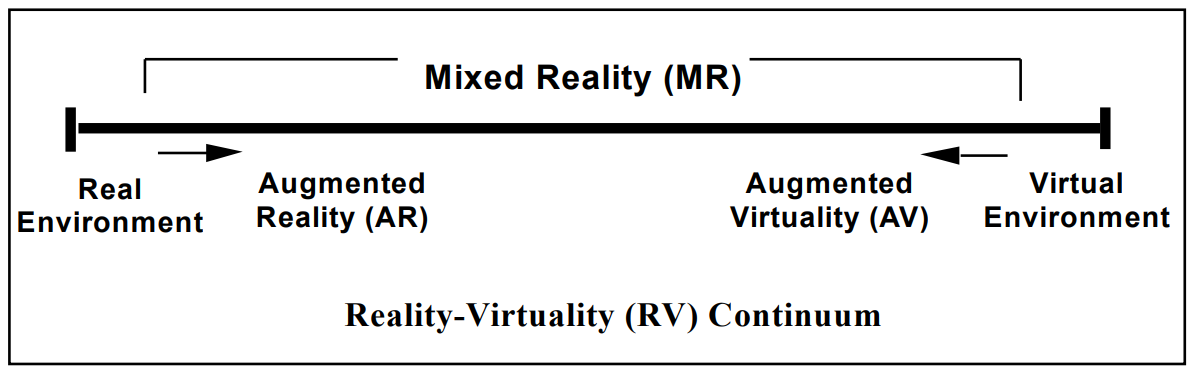
\includegraphics[scale=0.52]{ar_vr.png}
	\caption{Das Realität - Virtualität Kontinuum, Bildquelle \cite{ar_vr}}
\end{figure} 

Im Rahmen dieser Arbeit wird sich, wenn der Begriff Augmented Reality (AR) verwendet wird, auf Monitor basierte, nicht immersive Geräte bezogen, da sich in der Analyse der Verfahren und der Implementation einer AR Anwendung, auf Smartphones bezogen wird. Diese Anzeigesysteme werden auch als \glqq window-on-the-world\grqq{} bezeichnet, da computergenerierte Bilder oder Informationen digital über das Echtzeit Kamera Bild überlagert werden. (vgl. \cite{ar_vr} S.284)



\section{Augmented Reality - Software Development Kits}

\glqq Software Development Kits\grqq (SDK) oder auch Frameworks, sind Werkzeuge und Bibliotheken, welche eine Programmierumgebung und Basistechnologien liefern, um Programme zu entwickeln. Im Bereich von Augmented Reality SDKs umfassen Frameworks meistens die drei Hauptkomponenten: (vgl. \cite{sdks} S.3)

\begin{itemize}

\item \textbf{Recognition}: Erkennung von Bildern, Objekten, Gesichtern oder Räumen, auf welche die virtuellen Objekte oder Informationen überlagert werden können.


\item \textbf{Tracking}: Echtzeit-Lokalisierung der erkannten Objekte und Berechnung der lokalen Position des Gerätes zu diesen.

\item \textbf{Rendering}: Überlagerung der virtuellen Medieninformationen über das Bild und Anzeige der generieren Mixed Reality.
\end{itemize}

\subsection{Marktübersicht - SDKs}

\begin{itemize}

\item Vuforia
\item Wikitude
\item Metaio
\item ARToolKit
\item Kudan
\item EasyAR
\item MaxST
\item ARcore
\item ARKit

\end{itemize}



\section{Arten des Augmented Reality Trackings}

(Evtl bessere quellen für ref und hybrid)

\subsection{Referenzmarken-basiertes Tracking}

Markerbasiertes Tracking war lange Zeit eine der häufigsten verwendeten Techniken um Augmented Realtiy zu realisieren. Dies liegt in der einfachen Erkennung der typischerweise schwarz-weißen Marker mit hohem Kontrast. Dadurch kann neben der Relation des Geräts zum Marker auch relativ einfach die Entfernung und der Winkel berechnet werden. Der Nachteil liegt in der Limitierung der Anwendungsgebiete, in denen diese Technik verwendet werden kann, da Marker immer im Sichtfeld der Kamera lokalisiert sein müssen und nicht von anderen Objekten verdeckt werden dürfen. Weiterhin müssen immer externe Ressourcen verwendet werden um diese Marker zu erstellen und zu verwenden, was bei der Verbreitung der Anwendung immer mit einem Mehraufwand verbunden ist. (vgl. \cite{comparative_sdks} S.13)

\subsection{Hybrid-basiertes Tracking}

Hybrid basiertes Tracking verwendet mehrere Datenquellen wie das Global Positioning System (GPS), Kompass oder Beschleunigungssensoren zur Bestimmung der Orientierung und Lokalisierung des Geräts. Dabei wird per GPS der Standort des Geräts bestimmt, um Objekte in der Nähe zu identifizieren, die augmentiert werden sollen. Mit Hilfe des Kompasses kann dann ein Pfad erstellt und überprüft werden, ob die Orientierung des Geräts auch in diese Richtung zeigt. Der Beschleunigungssensor bestimmt die Ausrichtung des Geräts mithilfe der Gravitation. Durch die Vereinigung all dieser Informationen kann berechnet werden, was im Sichtfeld ergänzt werden soll, ohne dass eine Auswertung und Verarbeitung des realen aufgenommen Bildes stattzufinden hat. Anschließend werden die Informationen über das Kamerabild gelegt.  (vgl. \cite{comparative_sdks} S.13)

\subsection{Modell-basiertes Tracking}

Beim Modell-basiertem Tracking wird ein rekursiver Algorithmus verwendet. Hierbei wird die vorherige Kameraposition als Grundlage für die Berechnung der aktuellen Kameraposition verwendet. Durch die Rekursivität ist dieses Verfahren nicht sehr rechenintensiv und benötigt eine relativ geringe Prozessorleistung. Weiterhin kann zwischen verschiedenen Merkmalen unterschieden werden, welche für das Tracking verwendet werden. Bei der kantenbasierten Methode wird versucht ein dreidimensionales Wireframe mit den Kanten des Objekts in der realen Welt zuzuordnen

\begin{figure}[H]
	\centering
	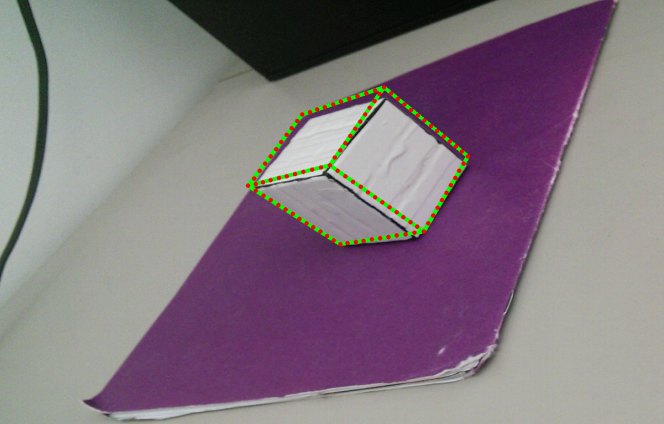
\includegraphics[scale=0.7]{wire.png}
	\caption{Kantenbasiertes rekursives Tracking, Bildquelle \cite{model_based} S.3}
\end{figure} 

Außerdem sind Ansätze wie \glqq optical flow based tracking\grqq{}, was zeitliche Informationen, entnommen aus der Bewegung der Projektion des Objekts relativ zur Bildebene verwendet, sowie texturbasierte Ansätze verbreitet. (vgl. \cite{model_based} S.1-2)



\subsection{Natürliches Feature Tracking}

Natürliches Feature Tracking ist ein bildbasiertes Verfahren und kann die Position des Gerätes zur Umgebung, ohne das Wissen über einen vorherigen Zustand bestimmen. Diese Methode ist in der Regel sehr rechenintensiv und benötigt hohe Prozessorleistung. (vgl. \cite{model_based} S.1-2) Diese Technik verwendet die Merkmale von Objekten in der echten Welt und erkennt die natürlichen Eigenschaften dieser. Diese Merkmale werden Features genannt und sind typischerweise, basierend auf einem mathematischem Algorithmus, sehr gut unterscheidbar und außern sich in der Form von Ecken, Kanten oder starke Kontrasten. Die Feature Deskriptoren eines Bildes werden zur späteren Erkennung gespeichert. Anhand des gespeicherten Datensets aus Merkmalen kann dann erkannt werden, ob ein Bild den gleichen Inhalt zeigt, unabhängig von Entfernung, Orientierung, Beleuchtungsintensität oder Verdeckung. (vgl. \cite{comparative_sdks} S.13) Es gibt eine Vielzahl an natürlichen Feature Tracking Systemen, wie SIFT (Scale-Invariant Feature Transform), SURF (Speeded Up Robust Features) oder \glqq Random Ferns\grqq{}. Diese unterscheiden sich hauptsächlich durch die Bildmerkmale zwischen Videobild und dem Modell der Umgebung die verfolgt werden soll. Die Grundsätzliche Pipeline kann wie in Abbildung 2.3 dargestellt, beschrieben werden.

\begin{figure}[H]
	\centering
	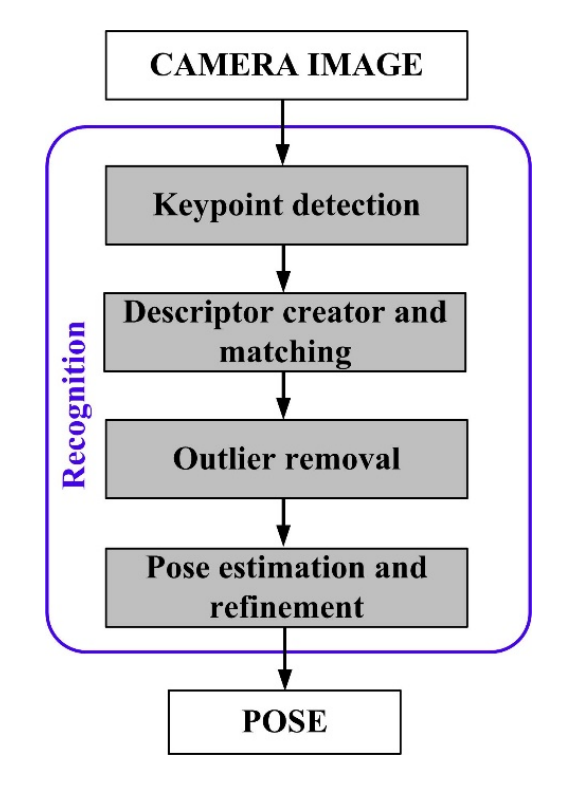
\includegraphics[scale=0.5]{tracking_pipeline.png}
	\caption{Tracking Pipeline Bildquelle \cite{natural_feature}}
\end{figure} 

Die Keypoint Erkennung wird normalerweise mit einer \glqq FAST corner detector\grqq{} bewerkstelligt.

\url{http://homepages.inf.ed.ac.uk/rbf/CVonline/LOCAL_COPIES/AV1011/AV1FeaturefromAcceleratedSegmentTest.pdf}

Die Erstellung und das Matching der Deskriptoren hängt von der Wahl des Deskriptors ab. Bei SIFT beispielsweise schätzt der Algorithmus die dominante Orientierung des Keypoints mit Hilfe von Gradienten, kompensiert die erkannte Orientierung und beschreibt abschließend die Keypoints in Bezug zu den Gradienten der Umgebung. Die erkannten Deskriptoren werden in eine Datenbank gespeichert, in welcher dann, während des Echtzeit Trackings, auf Gemeinsamkeiten geprüft werden kann. \glqq Outlier removal\grqq{} oder auch die Ausreißerbeseitigung besteht aus einer Reihe von Techniken zur Entfernung von unerwünschten, falsch erkannten Keypoints, beginnend mit günstigen Methoden (einfache geometrische Tests) und abschließend mit teuren, homographie basierten Tests. (vgl. \cite{natural_feature} S.28-29) 


Die planare Homographie bezieht sich auf die Transformation zwischen zwei Ebenen. Betrachtet man das erst Set and korrespondierender Punkte, $(x,y)$ im ersten Bild und $(x',y')$ im zweiten. Dann bildet die Homographie $H$ diese wie folgt ab.

\begin{equation}
  s  
  		\begin{bmatrix}
		x'\\
		y'\\
		1
     	\end{bmatrix}
     = H
     	\begin{bmatrix}
		x\\
		y\\
		1
     	\end{bmatrix}
      = 
     	\begin{bmatrix}
		h_11 & h_12 & h_13\\
		h_21 & h_22 & h_23\\
		h_31 & h_32 & h_33
     	\end{bmatrix}
      \
     	\begin{bmatrix}
		x\\
		y\\
		1
     	\end{bmatrix}
\end{equation}

Die Homographiematrix ist eine 3x3 Matrix mit 8 DoF (Degrees of Freedom). Sie wird standardmäßig normalisiert mit: 

\begin{equation}
h_33 = 1
\end{equation}

oder 
\begin{equation}
h²_{11} + h²_{12} + h²_{13} + h²_{21} + h²_{22} + h²_{23} + h²_{31} + h²_{32} + h²_{33} = 1
\end{equation}

Homographie wird in vielen Anwendungsbereichen, wie Panoramaerstellung, Bildausrichtung, perspektivischer Entzerrung oder für die Schätzung der Kameraposition in Augmented Reality verwendet. (vgl. \cite{homography})

Die verschiedenen Resultate der Homographie werden als Ausgangspunkt für die \glqq Pose Estimation\grqq (Positionsschätzung) verwendet.

\url{http://sci-hub.tw/10.1109/TVCG.2015.2513408}

 Abschließend wird, basierend auf dem Gauß-Newton-Verfahren eine Reduzierung des \glqq re-projection error\grqq{} erreicht. 
 
\url{https://mathepedia.de/Gausz-Newton-Verfahren.html} 
 
 Typischerweise sind zwei bis vier Wiederholungen genug. (vgl. \cite{natural_feature} S.28-29)


SIFT
SURF

\section{Warum beleuchte ich Photogrammetrie im Rahmen von AR}